% Copyright 2020 Glen Newton
% License: Creative Commons Attribution-ShareAlike 4.0 International License https://creativecommons.org/licenses/by-sa/4.0/legalcode
%\documentclass[a0paper,10pt]{article}
\documentclass[12pt]{article}


\usepackage{tikz}
\usepackage[margin=6mm]{geometry}

\usepackage[extreme]{savetrees}
\usepackage{microtype}
\usepackage[hidelinks]{hyperref}
\usetikzlibrary{mindmap,positioning}

%\usepackage{atbegshi}% http://ctan.org/pkg/atbegshi
%\AtBeginDocument{\AtBeginShipoutNext{\AtBeginShipoutDiscard}}


% from: https://tex.stackexchange.com/questions/250150/formatting-mindmap-in-tikz
\hypersetup{
  colorlinks=false
}

% from: https://tex.stackexchange.com/questions/107057/adjusting-font-size-with-tikz-picture

\begin{document}

\sffamily
\pagestyle{empty}

{\centering
  \noindent
  \makebox[0pt]{%
    \resizebox{\columnwidth}{!}
              {
                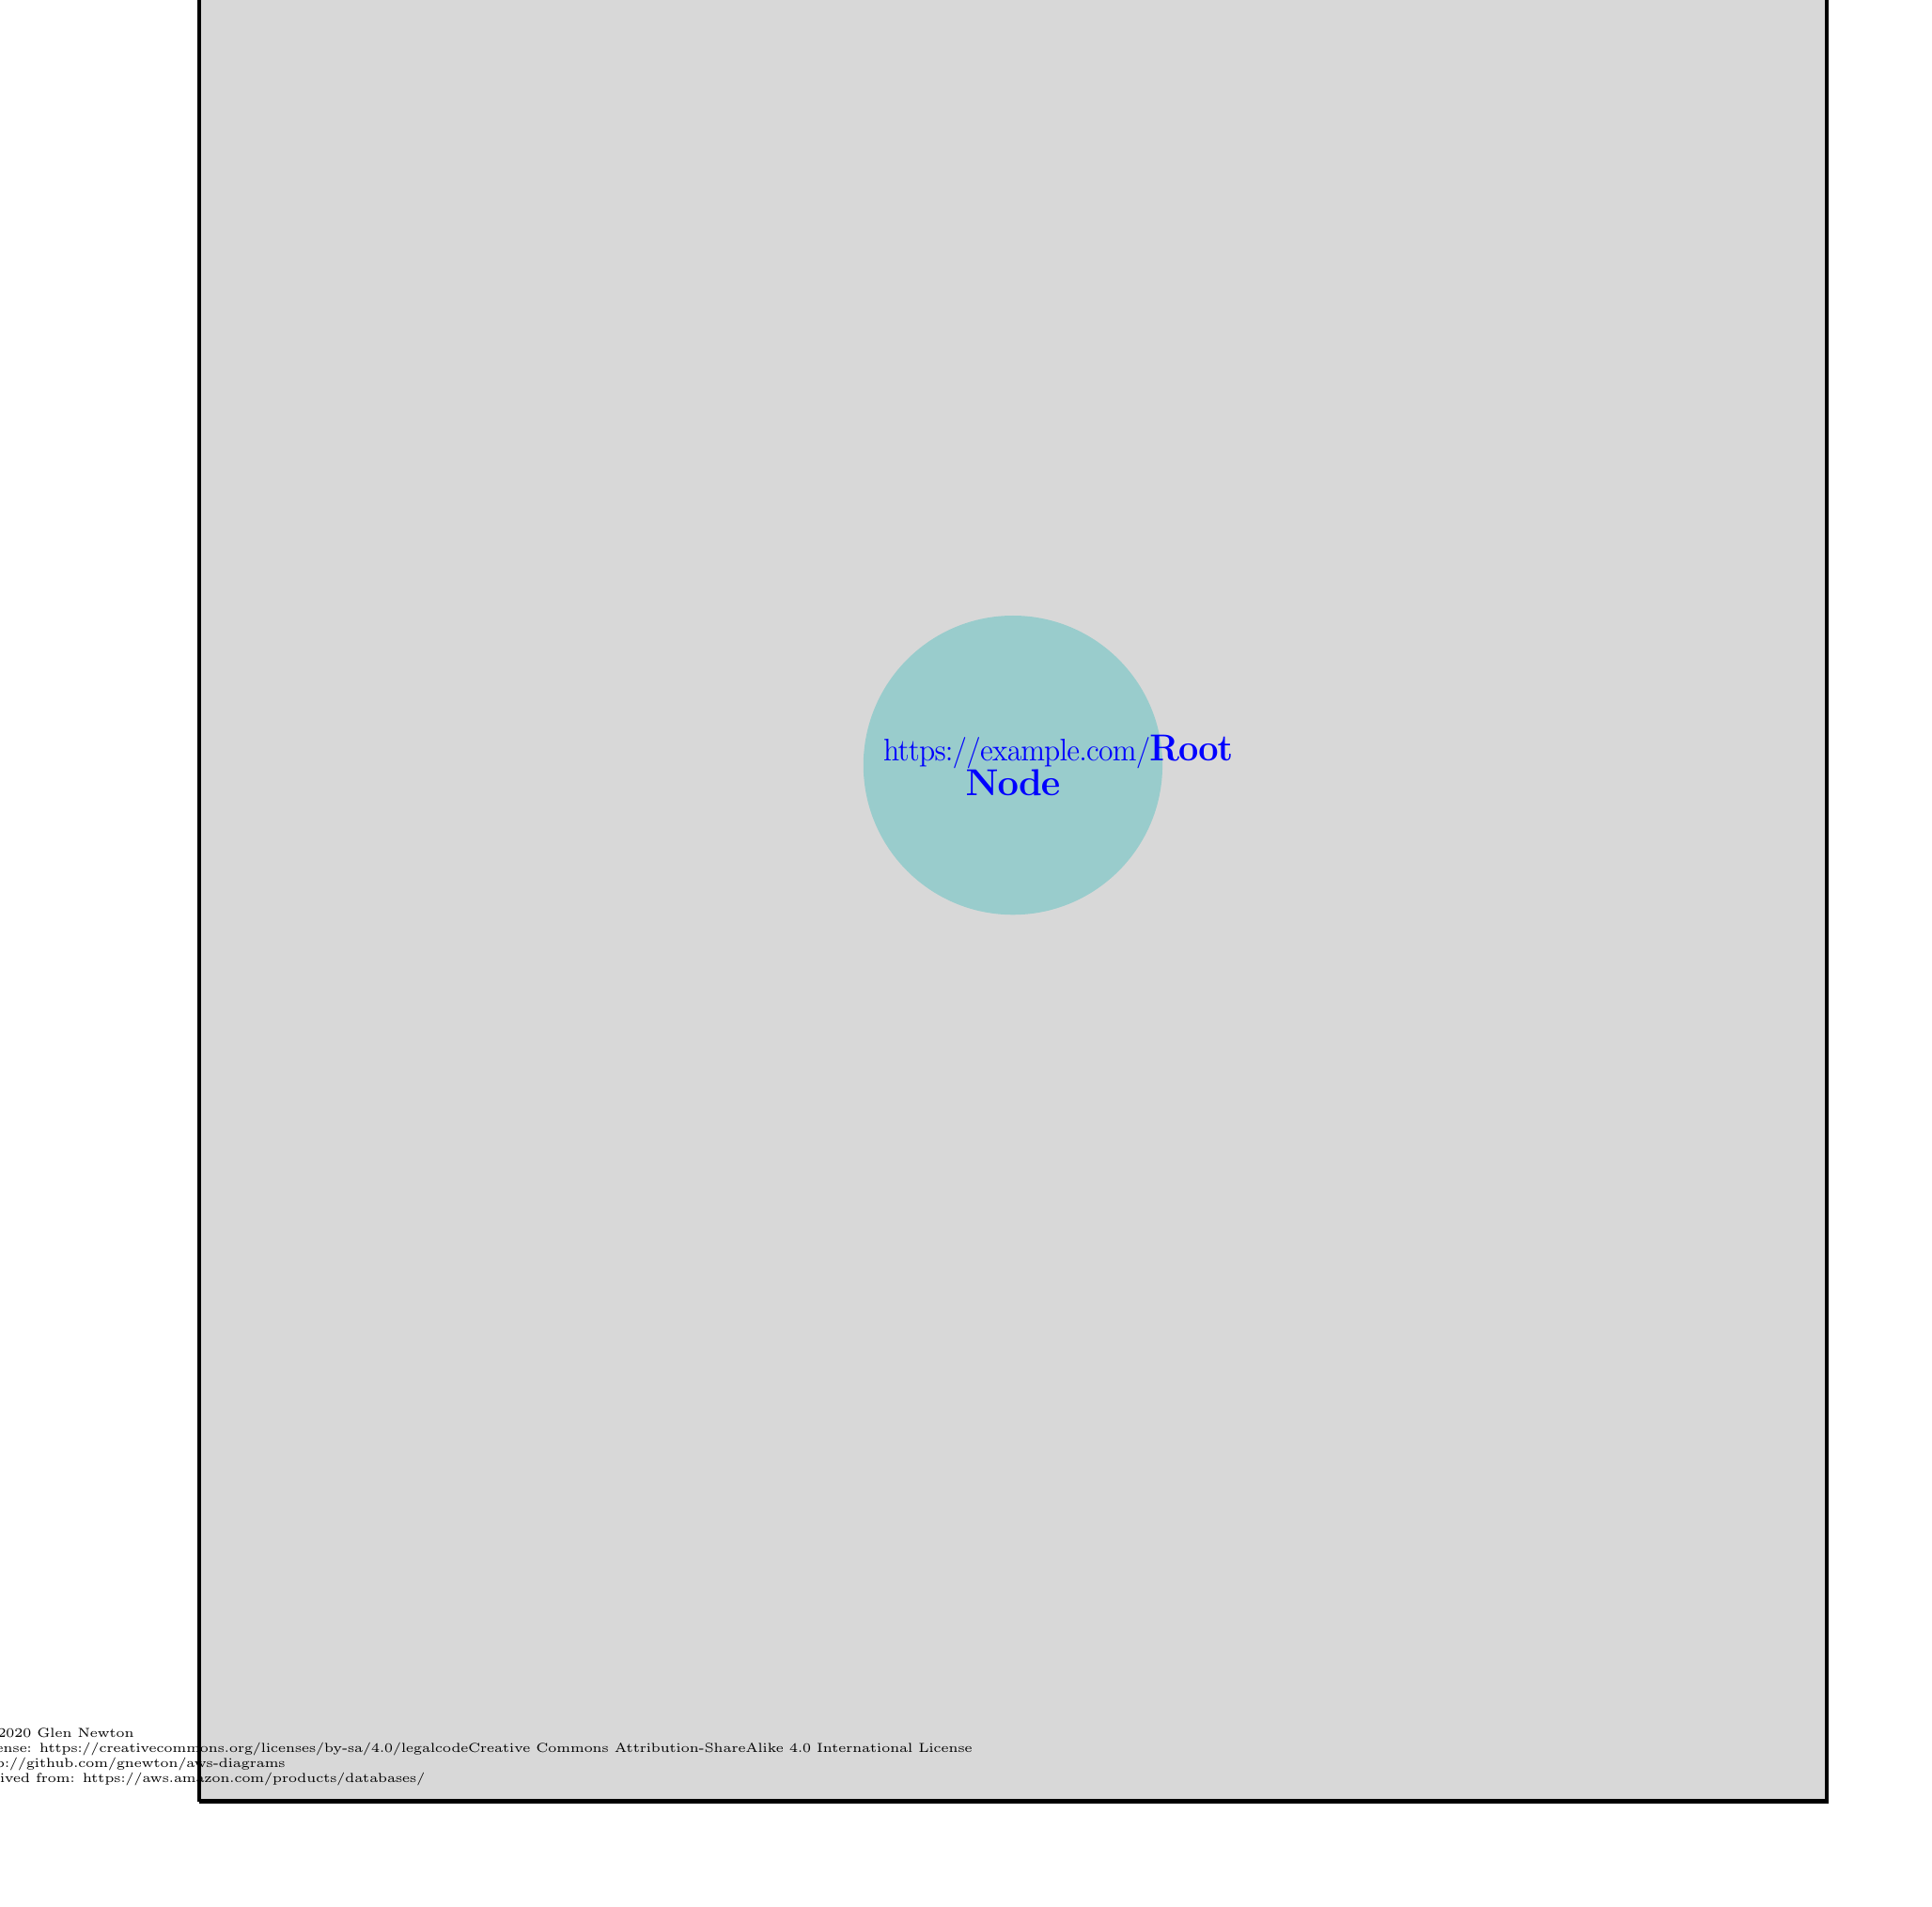
\begin{tikzpicture}
                  \begin{scope}
                    \draw [ultra thick, fill=gray!60, fill opacity=0.5] (-11,-14) -- (11,-14) -- (11,11) -- (-11,11) -- (-11,-14);
                  \end{scope}
                  \begin{scope}
                    [mindmap,
                      grow cyclic,
                      every node/.style=concept,
                      concept color=teal!40,
                      level 1/.append style={sibling angle=360/7, level distance=6.2cm,minimum size=3.2cm},
                      level 2/.append style={sibling angle=37.5, level distance=3.8cm,minimum size=2.3cm},
                      level 3/.append style={level distance=3cm,minimum size=1.4cm},
                    ]
                    \node [root concept] {\color{blue} \href{https://example.com/}{\Large \bfseries Root Node}};
                  \end{scope}
                    \node[xshift=-7.3cm,yshift=-13.3cm](foox) {
                      %                  Copyright 2020 Glen Newton
                                        \tiny
                  \begin{tabular}{l}
                  \\
                    \copyright \ 2020 Glen Newton\\
                    License: \href{https://creativecommons.org/licenses/by-sa/4.0/legalcode}{Creative Commons Attribution-ShareAlike 4.0 International License}\\
                    \url{http://github.com/gnewton/aws-diagrams} \\
                    Derived from: \url{https://aws.amazon.com/products/databases/}
                  \end{tabular}

                    };
  \end{tikzpicture}}}\par}


                \end{document}
